\documentclass[rgb,dvipsnames]{beamer}
\usepackage[english]{babel}
\usepackage{xcolor}
\usepackage{listings}
\usepackage{adjustbox}

\usepackage{amsmath}

\usepackage[linewidth=1pt]{mdframed}

% Graphics
\usepackage{graphicx}

% Font
\usepackage{paratype}
\setbeamerfont{frametitle}{family=\bf}
\usefonttheme[onlymath]{serif}

\newcommand{\nn}{\mathcal{N}}
\newcommand{\uu}{\mathcal{U}}
\newcommand{\bb}{\mathcal{B}}
\newcommand{\ee}{\mathrm{e}}
\newcommand{\rd}[1]{\mathrm{#1}}
\newcommand{\bd}[1]{\mathbf{#1}}  % for bolding symbols
\newcommand{\RR}{\mathbb{R}}      % for Real numbers
\newcommand{\ZZ}{\mathbb{Z}}      % for Integers
\newcommand{\BB}{\mathbb{B}}      % for Booleans
\newcommand{\PP}{\mathbb{P}}      % for Prob
\newcommand{\EE}{\mathbb{E}}      % for Expectation
\newcommand{\II}{\mathbbm{1}}      % for Indicator fun
\newcommand{\NN}{\mathbb{N}}      % for Prob
\newcommand{\col}[1]{\left[\begin{matrix} #1 \end{matrix} \right]}
\newcommand{\comb}[2]{\binom{#1^2 + #2^2}{#1+#2}}

\usepackage{tikz}
\usetikzlibrary{arrows,fit, positioning, shapes,
  calc, fadings, decorations.pathmorphing, hobby}

\tikzset{font=\tiny}
\tikzset{terminal/.style={circle, draw=black, fill=black, text=white}}
\tikzset{steiner/.style={circle, draw=black, fill=white}}
\tikzset{selected/.style={draw=red, ultra thick}}
\tikzset{assignment/.style={draw=red, thin, opacity=0.6}}
\tikzset{root/.style={draw=cyan, ultra thick}}
\tikzset{subgraph/.style={font=\large, text=gray}}
\tikzset{snake it/.style={-stealth,
    decoration={snake, 
      amplitude = .2mm,
    segment length = 2mm,
    post length=0.9mm},decorate}}
\tikzset{snake node/.style={above=1mm,
    midway,
    text width=3cm,
    sloped,
    align=center}}


% Beamer theme settings
\usetheme{Copenhagen}
\usecolortheme{seahorse}
\setbeamertemplate{itemize item}{\raisebox{0.8mm}{\rule{1.2mm}{1.2mm}}}
\usenavigationsymbolstemplate{} % no navigation buttons

\mode<presentation>
{ \usetheme{boxes} }

\title{Master's Thesis Defense}
\subtitle{The Prize-Collecting Steiner Tree Problem
  \\and Related Problems}
\author{William Jack Lysgaard Sprent}
\date{31st August 2018}
\institute{DIKU \\ University of Copenhagen}
\begin{document}

\AtBeginSection[]
{
   \begin{frame}
       \frametitle{Outline}
       \tableofcontents[currentsection]
   \end{frame}
 }
 
\frame{\titlepage}

\begin{frame}{The fun we are having today:}
\tableofcontents
\end{frame}

\section{Introduction}

\begin{frame}{Introduction}{Overview}
  \begin{block}{Initial Problem Statement}
    \textit{Apply results from research on the more covered Prize-Collecting Traveling Salesman
    Problem to the lesser covered Prize-Collecting Steiner Tree problem.}
  \end{block}
\end{frame}

\begin{frame}{Introduction}{Overview}
  \begin{block}{What I spent six months doing?}
  \pause
  \begin{itemize}
  \item I read a stack of research papers about the PCSTP.
  \item I read a smaller stack of research papers about problems related to the PCSTP. \pause
  \item \textit{I was indecisive.} \pause
  \item I worked on a solver for the Median Tree Problem.
  \end{itemize}
\end{block}
\end{frame}

\begin{frame}{Introduction}{Overview}
  \begin{block}{Revised Problem Statement}
    \textit{Apply results from research on the more covered Prize-Collecting Steiner Tree
      Problem to the lesser covered Median Tree Problem.}
   \end{block}
   \begin{block}{Goals}
     \begin{enumerate}
     \item Survey research on the PCSTP
     \item Identify methods worth \textit{porting}
     \item Implement these methods in a solver for the MTP
     \end{enumerate}
   \end{block}
\end{frame}

% \begin{frame}{Introduction}{Motivation}
%   \begin{block}{Why the PCSTP?}
%   \begin{itemize}
%   \item It is an NP-hard problem. Hard problems are worth solving.
%   \item It is typically solved using ILP.
%   \item It relates to the Steiner Tree Problem, and shares some of
%     its characteristica.
%     \pause
%   \item Finally: \textit{I think it is an interesting problem.}
%   \end{itemize}
% \end{block}

% \end{frame}

\begin{frame}{Introduction}{Motivation}
  \begin{block}{What makes a survey necessary?}
  \pause
  \begin{itemize}[<+->]
  \item A lot is written about the PCSTP, but it is unstructured and disjoint.
  \item Some of these papers touch on very complex subjects
    and are sometimes short and unintuitive.
  \item The PCSTP is a good ``case study'' for an Graph Optimisation and ILP problem.
  \end{itemize}
  \pause
  \textbf{ --- There is a lot to learn.}
\end{block}
\end{frame}

\begin{frame}{Introduction}{Motivation}
  \begin{block}{Why the Median Tree Problem?}
  \pause
  \textit{We'll get back to that later.}
\end{block}

\end{frame}
\section{The Prize-Collecting Steiner Tree Problem}
\begin{frame}{The Prize-Collecting Steiner Tree Problem}{Preface}
  \begin{block}{Short (Meta) History}
  \begin{itemize}[<+->]
  \item Defined by Egon Balas in 1988 as a side effect.
  \item Subject to steady focus in the late 90's and early 00's.
  \item One of the subjects of the 11th DIMACs Implementation Challenge in 2014.
  \end{itemize}
  \end{block}
\end{frame}
\begin{frame}{The Prize-Collecting Steiner Tree Problem}{Problem Definition}
 Given an undirected graph
\[G = (V, E, c, p)\]
where $c: E \to \RR^+$ defines edge weights,
and $p: V \to \RR^+$ defines vertex \textit{prizes}, then the solution to the
\textit{PCSTP} is a tree
\[T = (V_T, E_T, c, p) \subseteq G\]
which minimizes
\[c(T) = \min_T \sum_{(i,j) \in E_T} c_{ij} + \sum_{v\in (V \setminus V_T)} p_v \textnormal{.} \]
\end{frame}

\begin{frame}{The Prize-Collecting Steiner Tree Problem}{Example}
  \centering
  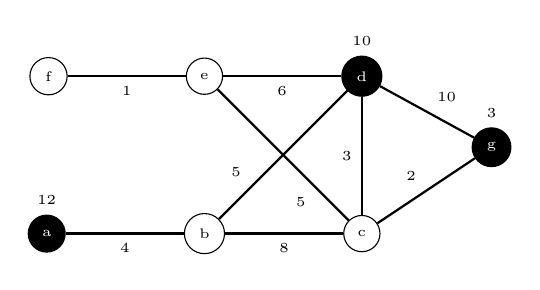
\begin{tikzpicture}[auto, node distance=1.5 cm]
  %Nodes
  \node[terminal, label={12}] (a) {a};
  \node[steiner] (b) [right=of a] {b};
  \node[steiner] (c) [right=of b] {c};
  \node[terminal, label={10}] (d) [above =of c] {d};
  \node[steiner] (e) [left=of d] {e};
  \node[steiner] (f) [left=of e] {f};
  \node[terminal, label={3}] (g) [above right=0.75 and 1.3 of c] {g};
  % Edges
  \begin{scope}[every edge/.style={draw=black, thick}]
    \draw (a) edge node[below]{4} (b);
    \draw (b) edge node[near start]{5} (d);
    \draw (b) edge node[below]{8} (c);
    \draw (c) edge node{3} (d);
    \draw (c) edge node{2} (g);
    \draw (c) edge node[near start]{5} (e);
    \draw (d) edge node{6} (e);
    \draw (d) edge node{10} (g);
    \draw (e) edge node{1} (f);
  \end{scope}
\end{tikzpicture}
\end{frame}

\begin{frame}{The Prize-Collecting Steiner Tree Problem}{Example}
  \centering
  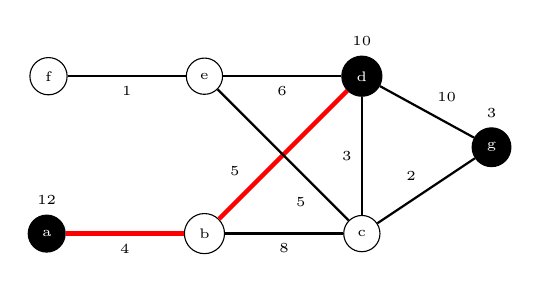
\begin{tikzpicture}[auto, node distance=1.5 cm]
  %Nodes
  \node[terminal, label={12}] (a) {a};
  \node[steiner] (b) [right=of a] {b};
  \node[steiner] (c) [right=of b] {c};
  \node[terminal, label={10}] (d) [above =of c] {d};
  \node[steiner] (e) [left=of d] {e};
  \node[steiner] (f) [left=of e] {f};
  \node[terminal, label={3}] (g) [above right=0.75 and 1.3 of c] {g};
  % Edges
  \begin{scope}[every edge/.style={draw=black, thick}]
    \draw (a) edge[selected] node[below]{4} (b);
    \draw (b) edge[selected] node[near start]{5} (d);
    \draw (b) edge node[below]{8} (c);
    \draw (c) edge node{3} (d);
    \draw (c) edge node{2} (g);
    \draw (c) edge node[near start]{5} (e);
    \draw (d) edge node{6} (e);
    \draw (d) edge node{10} (g);
    \draw (e) edge node{1} (f);
  \end{scope}
\end{tikzpicture}

\end{frame}

\section{The Survey}

\begin{frame}{The Survey}{Quick Summary}

  \begin{block}{Contents of the PCSTP Survey:}
  \begin{enumerate}
  \item The history of solving the PCSTP.
  \item Preprocessing routines.
  \item Two heuristic algorithms. LP-based and search based.
  \item An approximation algorithm: the GW Algorithm.
  \item How to separate GSECs.
  \item The DHEA and SCIP-Jack solvers.
  \end{enumerate}
\end{block}
\end{frame}

\begin{frame}{The Survey}{Main Points}
  \begin{block}{What have we learned?}
    \pause
    \begin{enumerate}
    \item The PCSTP is well covered all things considered. \pause
  \item Preprocessing is \textit{very} good for the PCSTP. \pause
  \item Directed formulations of the problem are preferable for
    branch and bound. \pause
  \item Heuristics are aplenty.
  \end{enumerate}
  \end{block}

\end{frame}

\begin{frame}{The Survey}{Main Points}
  \begin{block}{Curiosities} \pause
  \begin{itemize}
  \item Not a lot of focus on applications
  \item Linear progress turns to lateral progress
  \item Somewhat general methods besides preprocessing
  \end{itemize}
\end{block}
\pause
\textit{On to other problems.}
\end{frame}

\begin{frame}{The Survey}{Prize-Collecting Tours}
  \begin{block}{Three main variants:}
    \begin{enumerate}
    \item The Prize-Collecting Travelling Salesman Problem
    \item The Orienteering Problem
    \item The Profitable Tour Problem
    \end{enumerate}
  \end{block}
  \pause
  \begin{block}{Some Notes:}
  \begin{itemize}
  \item Main point of the Balas paper in 88
  \item Shares approximation algorithms
  \item Apart from the OP, not well covered
  \end{itemize}
\end{block}

\end{frame}

\begin{frame}{The Survey}{Median Subgraphs}
  \begin{block}{Notes}
    \begin{itemize}
    \item Assignment Problem
    \item Different shapes of facility
    \item Median Trees are only research on shaped graphs
  \end{itemize}
\end{block}
\end{frame}

\begin{frame}{The Survey}{Related Problems}
  \begin{block}{Summary}
  \begin{itemize}
  \item Two axes of similarity: structure of solution and type of prize function
  \item PCSTP is the most well researched problem in the family
  \end{itemize}
\end{block}
\end{frame}

\section{The Median Tree Problem}
\begin{frame}{Median Tree Problem}{Motivation}
  \textit{Question: How do I best make use of the survey?} \pause
  \begin{block}{Options}
  \begin{itemize}[<+->]
  \item Stay with the PCSTP
  \item Look at the Profitable Tour Problem
  \item Look at the Median Tree Problem
  \end{itemize}
  \end{block}
\end{frame}

\begin{frame}{Median Tree Problem}{Motivation}
  \begin{block}{Median Trees instead of Prize-Collecting Tours}
    \begin{itemize}
    \item A feasible solution to the PCSTP is a feasible solution to the MTP
    \item Collect Prize vs. Assignment: similar --- although not the exact same --- trade offs
    \end{itemize}
    \pause
    \textit{And, of course, a splash of subjectivity.}
  \end{block}
\end{frame}

\begin{frame}{Median Tree Problem}{Problem Definition}
  Let $G = (V, E, c, d)$ be an undirected graph. Denote $c : E \to \RR^+$ as an \textit{edge cost} function
and $d : V \times V  \to \RR^+$ be an \textit{assignment cost} function where we have
\[d_{ii} = 0 \mathnormal{.}\]
Then the \textit{Median Tree Problem}
is defined as finding a \textit{connected subgraph} $T = (V_T, E_T)$ of $G$
where $V_T \subseteq V$ and
$E_T \subseteq E$ which minimises the cost function,
\[c(T) = \sum_{ij \in E_T} c_{ij} + \sum_{i \in V} \min_{j \in V_T} d_{ij}\mathnormal{.}\]
\end{frame}

\begin{frame}{Median Tree Problem}{Example}
  \centering
      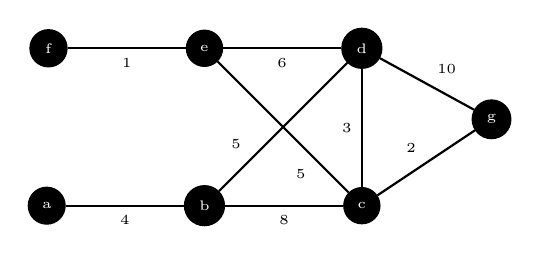
\begin{tikzpicture}[auto, node distance=1.5 cm]
      % Nodes
      \node[terminal] (a) {a};
      \node[terminal] (b) [right=of a] {b};
      \node[terminal] (c) [right=of b] {c};
      \node[terminal] (d) [above =of c] {d};
      \node[terminal] (e) [left=of d] {e};
      \node[terminal] (f) [left=of e] {f};
      \node[terminal] (g) [above right=0.75 and 1.3 of c] {g};
      % Edges
      \begin{scope}[every edge/.style={draw=black, thick}]
        \draw (a) edge node[below]{4} (b);
        \draw (b) edge node[near start]{5} (d);
        \draw (b) edge node[below]{8} (c);
        \draw (c) edge node{3} (d);
        \draw (c) edge node{2} (g);
        \draw (c) edge node[near start]{5} (e);
        \draw (d) edge node{6} (e);
        \draw (d) edge node{10} (g);
        \draw (e) edge node{1} (f);
      \end{scope}
    \end{tikzpicture}

\end{frame}

\begin{frame}{Median Tree Problem}{Example}
  \centering
  \begin{tabular}{r||c|c|c|c|c|c|c}
 $d_{ij}$ & $a$ & $b$ & $c$ & $d$ & $e$ & $f$ & $g$ \\ \hline\hline
      $a$ &  0  &  12 &  12 &  12 &  12 &  12 &  12 \\ \hline
      $b$ &  0  &  0  &  0  &  0  &  0  &  0  &  0  \\ \hline
      $c$ &  0  &  0  &  0  & 0  &  0  &  0  &  0  \\ \hline
      $d$ &  10 &  10 &  10 &  0  &  10 &  10 &  10 \\ \hline
      $e$ &  0  &  0  &  0  &  0  &  0  &  0  &  0  \\ \hline
      $f$ &  0  &   0 &  0  &  0  &  0  &  0  &  0  \\ \hline
      $g$ &  3  &   3 &  3  &  3  &  3  &  3  &  0
  \end{tabular}

\end{frame}

\begin{frame}{Median Tree Problem}{Example}
  \centering
    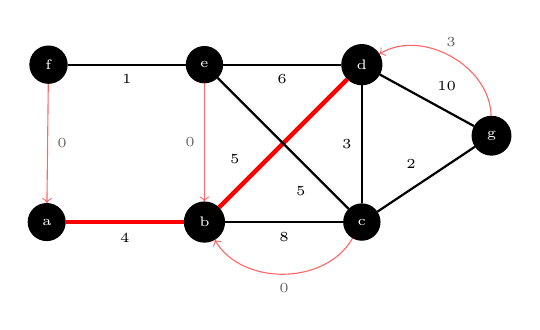
\begin{tikzpicture}[auto, node distance=1.5 cm]
      % Nodes
      \node[terminal] (a) {a};
      \node[terminal] (b) [right=of a] {b};
      \node[terminal] (c) [right=of b] {c};
      \node[terminal] (d) [above =of c] {d};
      \node[terminal] (e) [left=of d] {e};
      \node[terminal] (f) [left=of e] {f};
      \node[terminal] (g) [above right=0.75 and 1.3 of c] {g};
      % Edges
      \begin{scope}[every edge/.style={draw=black, thick}]
        \draw (a) edge[selected] node[below]{4} (b);
        \draw (b) edge[selected] node[near start]{5} (d);
        \draw (b) edge node[below]{8} (c);
        \draw (c) edge node{3} (d);
        \draw (c) edge node{2} (g);
        \draw (c) edge node[near start]{5} (e);
        \draw (d) edge node{6} (e);
        \draw (d) edge node{10} (g);
        \draw (e) edge node{1} (f);
      \end{scope}
      \begin{scope}[every edge/.style={assignment}]
        \draw[->] (c) edge[bend left=60] node{0} (b);
        \draw[->] (e) edge node[left]{0} (b);
        \draw[->] (f) edge node{0} (a);
        \draw[->] (g) edge[bend right=60] node[above]{3} (d);
      \end{scope}
    \end{tikzpicture}
\end{frame}

\begin{frame}{Median Tree Problem}{ILP Formulation}
  \begin{subequations}
    \small
     \begin{alignat}{3}
       &\underset{\bd x, \bd y}{\text{minimize}}
       & & \sum_{ij \in E} c_{ij} x_{ij} +  \sum_{i, j \in V} d_{ij}y_{ij}  & \\
       & \text{subject to}\quad
       & & \sum_{ij \in E} x_{ij} = \sum_{i \in V} y_{ii} - 1 &&  \label{form:mtp:tree}\\
       &&& x(E(S)) \leq \sum_{i \in S \setminus \{s\}} y_{ii}
       && \forall S \subseteq V, s \in S \label{form:mtp:gsec} \\
       &&& \sum_{j \in V} y_{kj} = 1 && \forall k \in V \label{form:mtp:assignment}\\
       &&& y_{ik} \leq  y_{kk}
       && \forall i, k \in V \label{form:mtp:facility}\\
       &&& y_{kk} \leq \sum_{i \in \delta(k)} x_{ik}
       && \forall k \in V \label{form:mtp:legal} \\
       &&& \bd x \in \BB^{|E|} && \\
       &&& \bd y \in \BB^{|V \times V|}
     \end{alignat}
   \end{subequations}
 \end{frame}
    \normalsize
 \begin{frame}{Median Tree Problem}{Valid Inequalities}
\pause
\textit{Forced self-assignment:}
\[
 y_{ii} \geq x_{ji} \qquad \forall i \in V,  \forall j \in \delta(i)\mathnormal{.}
\]
\pause
\textit{Degree of Nonterminals:}
\[
   \sum_{j \in \delta(i)}x_{ij} \geq 2 x_{ik} \qquad \forall i \in N, \: \forall k \in \delta(i)
\]
 \end{frame}

 \begin{frame}{Median Tree Problem}{The Solver}
 \begin{block}{Specifications}
   \begin{itemize}
   \item Based on the Gurobi MIP solver. \pause
   \item Callbacks written in Python 3. \pause
   \item Applies methods from the PCSTP survey: \pause
    \begin{itemize}
    \item Primal heuristic from the DHEA solver.
    \item User cuts based on GSEC separation from an
      article by Lucena and Resende for the PCSTP.
    \end{itemize}
  \end{itemize}
  
\end{block}

\end{frame}

\begin{frame}{Median Tree Problem}{Computational Experience}
  \begin{block}{Results}
    \pause
    \begin{itemize}[<+->]
    \item Primal Heuristics: Ambivalent performance
    \item Valid Inequalities: Ambivalent performance
    \item User Cuts: \textit{Terrible} performance
    \end{itemize}
  \end{block}
  \pause
  \textit{Why?}
\end{frame}

\section{Reflections}
\begin{frame}{Reflections}{Summary}
  \begin{block}{What did I manage to do?}
    \begin{itemize}
    \item Survey of the PCSTP
    \item ILP formulation for the MTP
    \item Dataset for the MTP
    \item Solver for the MTP
    \end{itemize}
  \end{block}
\end{frame}

\begin{frame}{Reflections}{Improvements}
  \begin{block}{Survey criticism}
    \begin{itemize}[<+->]
    \item I approach approximation algorithms, exact algorithms, and heuristics the same way
    \item I spend too much time with a ``zoomed in'' perspective
    \item More figures outside the preprocessing section
    \item Too little focus on application -- may be a feature of the body of research
    \end{itemize}
  \end{block}
\end{frame}

\begin{frame}{Reflections}{Improvements}
  \begin{block}{Solver section criticism}
    \begin{itemize}[<+->]
    \item Python is fun and fast for me, but slow for the PC
    \item Something is deeply wrong with the GSEC seperation routine
    \item I should have measured performance in other ways than end to end execution time
    \item The dataset is a bit uninteresting
    \end{itemize}
  \end{block}\pause
  \textbf{Overall: slight lack of a red thread}
\end{frame}


\begin{frame}{Reflections}{Lessions Learned}
  \begin{block}{Thoughts about the subject field}
    \begin{itemize}[<+->]
    \item There is a limit on how much research on an arbitrary problem is interesting
      without real world motivation
    \item Same with laterally defining new problems
    \item There could be a greater focus on generalising
      results as widely as possible
    \end{itemize}
  \end{block}
\end{frame}

\begin{frame}{Reflections}{Further Work}
  \begin{block}{Make the solver as good as it can be}
    \textit{Perform a more thorough investigation of the shortcomings in the MTP
    solver, and use these results to reimplement the solver.}
  \end{block}

  \begin{block}{Apply}
    \textit{Operationalise the research done on the PCSTP (or MTP) for a real-world
    problem field, and apply it to a specific scenario.}
  \end{block}
\end{frame}

% \begin{frame}{Reflections}{Lessions Learned}
%   \begin{block}{Personal lessions}
%     \begin{itemize}[<+->]
%     \item Learn to plan ``exploratoratively''
%     \item Have a product in sight much earlier
%     \item Working without application is demotivating 
%     \end{itemize}
%   \end{block}
% \end{frame}

\begin{frame}{Postface}
  \pause
  \large\textbf{Questions?}
\end{frame}
\end{document}